\chapter{Grundlegende Begriffe}
\label{ch:basics}
In folgendem Kapitel werden die Grundlagen erläutert, welche für spätere Kapitel benötigt werden. 
Es wird kurz auf die Historie von Turing Tests eingegangen, 
bevor die verschiedenen CAPTCHA-Methoden und Alternativen grundlegend erläutert werden. 
Zuletzt wird ein grundlegendes Verständnis für UX geschaffen.

\section{Turing Tests}
\label{ch:basics:turing}
Alan M. Turing $($1912-1954$)$ ist einer der Mitbegründer der heutigen Informatik 
und legte mit seiner Forschung einen der Grundsteine für die Entwicklung von künstlicher Intelligenz. 
In seinem Paper ''On computable numbers, with an application to the Entscheidungsproblem'' \cite{turing} 
beschreibt er den Umgang mit ''computable numbers'' und wie diese durch eine - später als Turing Machine bezeichnete - Maschine berechnet werden könnte.
Diese Turing Machine ''[\dots] ist damit ein Model physischer digitaler Computer, die zu jener Zeit jedoch noch nicht existieren. [\dots]'' \cite[p.4]{pallay2020turing}
Hierbei kam er zur Erkenntnis, dass sich nicht alle mathematischen Probleme durch eine fixe Vorgehensweise, also einen Algorithmus, lösen lassen. 
Erst später wurde festgestellt, dass Turing Maschinen und Computer jeweils vom anderen simuliert werden können. \cite[p.647]{geniusofturing} \cite[p.4]{pallay2020turing} %TODO: Formulierung

Turing beschäftigte sich bis zu seinem frühen Tod weiterhin mit maschineller Intelligenz 
und ''[\dots] beschreibt [\dots] das, was man heute als [\dots] künstliche Intelligenz bezeichnet.'' \cite[p.10]{pallay2020turing}
Durch seine Überzeugung, dass eines Tages maschinelle Intelligenzen entwickelt werden (können), 
entwickelte Turing in seinem Paper ''Computing Machinery and Intelligence'' \cite[p.23ff]{turing2009computing} 
eine Methode des Testens der Intelligenz einer Maschine. 
Um die Notwendigkeit von genauen Definitionen zu vermeiden, nutzt er deshalb ein Abwandlung eines Verfahren - des ''imitation games''. 
''Hierbei kommuniziert ein Juror maschinen-schriftlich mit einem Menschen und einer Maschine.'' \cite[p.12]{pallay2020turing}
Sollte der Juror nicht feststellen können, welcher Gesprächspartner der Mensch ist, gilt der Test als bestanden. \cite[p.11ff]{pallay2020turing}

Dieses Verfahren wird heute oftmals als Turing Test bezeichnet. 

\section{CAPTCHA}
%label
Bei der Abkürzung CAPTCHA handelt es sich um ''completely automated public turing tests to tell computers and humans apart''. 
Sie werden genutzt, um Webseiten vor Angriffen durch Bots zu schützen. 
Dies wird durch die im vorherigen Kapitel bereits erläuterten Turing Tests erreicht. 
Hier ist das Ziel, durch für Computer schwer, für Menschen jedoch leicht zu verarbeitende Medien, das Tracken von Mausbewegungen
oder das Prüfen der Browseraktivität zu prüfen, ob es sich wirklich um eine*n menschliche*n Nutzer*in handelt.

Fast identisch zu CAPTCHA sind sogenannte HIP – ''Human Interactive Proofs''. 
Dieser Begriff hat sich entwickelt, da manche Tests nicht ''public'' sind. \cite[p.1]{chellapilla} \cite{tutorial} 

\subsection{Arten von CAPTCHA}
%Nachfolgend werden verschiedene Arten von CAPTCHAs grundlegend erläutert.

Textbasierte CAPTCHA waren bereits 2008 die am häufigsten verwendete Art von CAPTCHA.
Sie zeichnen sich durch eine Verzerrung eines Wortes oder mehreren Wörtern aus, sodass diese für Bilderkennungstools nicht erkennbar sind.
Eine weitere Variante textbasierter CAPTCHA ist die einer einfachen Rechenaufgabe. 
Auch hier soll erreicht werden, dass ein Bot die angegebenen Zahlen nicht korrekt erkennen kann und die Gleichung somit nicht lösen kann. \cite{usabilityofcaptchas} \cite[p.75]{surveyofresearch} \cite{shinde2018DIFFERENTTO} %TODO SEITEN!!!!!!!!!

Bei der Darstellung dieser Zeichen und Symbole können verschiedene Ansätze verfolgt werden.
\citeauthor{surveyofresearch} beschreiben hierbei ``anti-segmentation techniques'' und ``anti-recognition techniques''. \cite[p.76]{surveyofresearch}

Anti-Segmentation Techniques zielen darauf ab, das Separieren der einzelnen Buchstaben durch Algorithmen zu erschweren. 
Um dies zu erreichen, gibt es verschiedene Herangehensweise.
Eine von ihnen besteht daraus, dass nur die Konturen der verschiedenen Zeichen angezeigt werden, sodass diese nur von Menschen erkannt werden können,
Bots hingegen wenig Chancen haben, diese korrekt zu unterscheiden. Diese Art von CAPTCHA nennen \citeauthor{surveyofresearch} ``Hollow CAPTCHAs''. %Formulierung
Eine weitere Methode ist, Zeichen nah beieinander oder sogar überlappend darzustellen, 
was von \citeauthor{surveyofresearch} als ``crowing characters together $($CCT$)$ and overlapping'' bezeichnet wird.
Auch unruhige Hintergründe können Segmentierung behindern.
Ebenfalls beschrieben wird die Kombination von mehreren der beschriebenen CAPTCHAs zu einer ``two-layer'' Struktur,
wobei die Tatsache, dass es sich um mehrere Zeilen Text handelt, nicht erkannt werden kann.

Anti-Recognition Techniques sind zum Beispiel verschiedene Schriftarten, die Rotation von Zeichen und ``Waving'', 
welche es erschweren, Zeichen als solche zu erkennen. 
Außerdem können in einigen Fällen auch sehr große Zeichensätze, beispielsweise Mandarin oder Japanisch, genutzt werden, 
wodurch das Finden von eindeutigen Lösungen erschwert werden kann.
Diese Techniken werden oftmals miteinander kombiniert.
\cite{surveyofresearch}

\begin{figure}
    \centering
    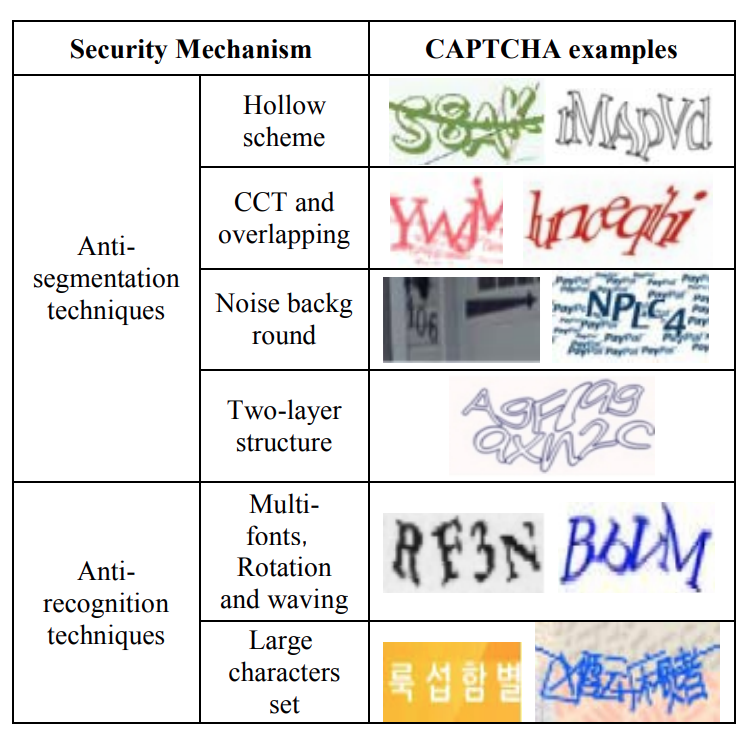
\includegraphics{gfx/mygraphics/unbedingtaustauschen1.png}
    \caption{textbasierte Beispiele die ich unbedingt noch austauschen muss, weil sie aus \cite{surveyofresearch} sind}
\end{figure}

A. Selection-based CAPTCHA
The users are required to select the correct answers
according to a hint for selection-based CAPTCHAs. It is the
simplest form of an image-based CAPTCHA. Several
examples of selection-based CAPTCHA are shown in Fig. 2.
Fig. 2. Examples of selection-based CAPTCHAs
The Asirra CAPTCHA [27] asks users to select all the
photographs with cats out of 12 photographs. This type of
CAPTCHA was the first attempt at an image-based
CAPTCHA. In contrast, the SEMAGE (SEmantically
MAtching imaGEs) CAPTCHA [32] asks users to select
semantically related images from a given image set. This type
of CAPTCHA exploits the ability of humans to accurately
understand image content and establish semantic relationships
between them. Avatar CAPTCHA is proposed in [59]. It asks
users to identify avatar faces from a set of 12 grayscale
images. The FR-CAPTCHA [33] and the FaceDCAPTCHA
[34] are face-based CAPTCHAs relying on human face
recognition. FR-CAPTCHA asks users to select two face
images of the same person. FaceDCAPTCHA requires users
to distinguish the visually distorted real human faces among
nonhuman face images. The Google CAPTCHA asks users to
select all images with street signs or some specific object. The
Facebook CAPTCHA asks users to select the corresponding
images directly, according to a hint, from twelve images with
different content. Recently, the work in [75] even construct a
more sophisticated image CAPTCHA method by using
semantic correlation to connect question keywords with
answer choices.
Golle [28] proposed an SVM (Support Vector Machine)
classifier to distinguish the images of cats and dogs in Asirra
with an 82.7% success rate. In [36], Gao’s team utilized
OpenCV functions to detect faces in the FR-CAPTCHA, and
four features were extracted from the faces to find the most
probable pair. Reference [39] leveraged deep learning
technologies to break an image reCAPTCHA and the
Facebook CAPTCHA with success rates of 70.78% and
83.5%, respectively.
Selection-based CAPTCHAs are simple and convenient
for users to operate. However, they have gradually become
vulnerable due to the development of deep learning.
B. Click-based CAPTCHA
In 2008, Richard Chow et al.[23] first proposed the clickbased CAPTCHA. It requires users to click characters in a
complex background according to a short hint, as shown in
Fig. 3. This CAPTCHA simplifies the user's operation,
shortens the passing time and minimizes users’ frustration.
Fig. 3. Examples of click-based CAPTCHAs
In general, click-based CAPTCHAs have two defense
mechanisms: anti-detection and anti-recognition. It is no
longer a difficult task to recognize characters correctly with
the development of machine learning. Therefore, almost all
security mechanisms focus on preventing attackers from
77
Authorized licensed use limited to: Fachhochschule FH Darmstadt. Downloaded on July 29,2022 at 08:34:41 UTC from IEEE Xplore. Restrictions apply.
correctly detecting characters. As shown in Fig. 3(c), the
CAPTCHA uses the style transfer technique [24] to embed
characters into the background to achieve the effect of hiding
the characters.
Recently, a novel click-based CAPTCHA named VTT was
proposed by Tencent (see Fig. 4). For a computer, it is
difficult to understand the semantic information and analyze
the image content as well as humans. In this regard, it seems a
good design. However, state-of-the-art research on visual
reasoning, such as [58] and [8], may break this scheme in the
near future.
Fig. 4. Examples of VTT CAPTCHAs
C. Drag-based CAPTCHA
The drag-based CAPTCHA judges whether the user is a
human through the mouse’s track, speed and response time.
The operation of a drag-based CAPTCHA is simple. Some
drag-based CAPTCHAs are shown in Fig. 5.
Fig. 5. Examples of drag-based CAPTCHAs
The What’s Up CAPTCHA, proposed by Google [37], is
the first drag-based CAPTCHA. Users need to identify the
upright orientations of randomly rotated images and adjust
them to the correct position. Setting an image to an upright
orientation is easy for humans, whereas it is difficult for bots.
It is worth noting that images used in CAPTCHA must be
manually filtered from of samples that do not contain clear
directional information. After this development, GeeTest
proposed the first version of a slider CAPTCHA. Users must
drag a slider along a line to the specified position
continuously. Inspired by this, the VAPTCHA appeared. It
asks users to draw a trajectory with a mouse according to an
arrow trajectory embedded in the background.
In fact, early drag-based CAPTCHAs judged the
legitimacy of users only by measuring the speed of their
operation. Therefore, it can be easily imitated. The later dragbased CAPTCHAs usually incorporate some user background
data analysis. At present, this seems to be the future
development trend for CAPTCHAs

Es gibt verschiedene Arten von bildbasierten CAPTCHAs. 
Die wohl bekannteste ist ein in Quadrate aufgeteiltes Bild, wobei man jene Quadrate auswählen soll, welche einen bestimmten Gegenstand enthalten.
Eine Variation dieses CAPTCHAs besteht aus einer Zahl verschiedener Bilder, von denen eine Teilmenge ebenfalls ein gesuchtes Objekt beinhalten.
%Discord CAPTCHA: PFERDE AUS WOLKEN!!!!!
Eine Form von bildbasierten sind Gamification captcha

%Audiobasiert

A. Audio-based CAPTCHA
This CAPTCHA is usually considered an alternative to a
visual CAPTCHA in the case of visually impaired users [44].
Users in most audio-based CAPTCHAs play the role of
listeners, and they are required to complete the specified
challenge based on what they have heard. A spoken
CAPTCHA system was introduced in [45]. This system
converts a selected word into speech using a Text-To-Speech
(TTS) system, then plays the sound clip to users and asks them
to say the word. In 2012, the SoundsRight audio CAPTCHA
(Fig. 6(a)) provided in [48] asks users to identify a specific
sound, such as the sound of a bell or a piano. This work has
increased the success rates in audio Captchas from less than
50% to over 90% for blind users. Meutzner et al. presented a
new type of audio CAPTCHA [50] that uses additional
nonsense speech sounds that are confusing for speech
recognizers, while being less critical for human listeners. In
2016, they also proposed a nonspeech audio CAPTCHA [61],
which is entirely based on the classification of sound events
mixed into an environmental scene. Moreover, the HuMan
CAPTCHA designed in [60] asks users to answer the
presented questions by combining ambient noise and common
sense knowledge. There is another type of audio-based
CAPTCHA in which users play the role of speakers and are
required to pronounce rather than simply listen. For instance,
Gao et al. [47] proposed a new sound-based CAPTCHA (Fig.
6(b)) that exploits the differences between a human voice a
synthetic voice. A user is required to read out a given sentence
rather than listening an audio file.
Fig. 6. Examples of audio-based CAPTCHAs
Attack and defense always go together. A two-stage attack
for the listener model can always obtain a good attack result.
In detail, the audio-based CAPTCHA is segmented into
several regions regarding the location of each spoken word
first. Then, the regions are recognized by automatic speech
recognition programs. Tam et al. achieved success rates of up
to 71% (Google Audio CAPTCHA, reCAPTCHA Audio
CAPTCHA, Digg CAPTCHA)[44]. Bursztein et al. achieved
success rates of 45%, 49% and 83% on the CAPTCHAs of
Yahoo, Microsoft and eBay, respectively[49]. Some
78
Authorized licensed use limited to: Fachhochschule FH Darmstadt. Downloaded on July 29,2022 at 08:34:41 UTC from IEEE Xplore. Restrictions apply.
researchers have even proposed that most of the digit-based
audio CAPTCHAs are successfully broken with success rates
between 50%-90% [44][52][54].
B. Video-based CAPTCHA
In video-based CAPTCHAs, users are provided a video
file, and they should choose one option that best matches the
video. Motion CAPTCHAs (Fig. 7(a)) proposed in [46] asks
users to select the sentence that describes the motion of the
person in the video. Rao et al. [55] proposed a video
CAPTCHA (Fig. 7(b)) based on advertisement recognition.
Both CAPTCHAs need users to select from the options
provided. That is, these schemes can be broken by random
guessing. Contrastly, reference [42] presented a video-based
CAPTCHA (Fig. 7(c)), which asks users to type three words
that best describe a video.
Fig. 7. Examples of video-based CAPTCHAs
Due to recent advances, bandwidth and video analysis
technology no longer limit the development of video-based
CAPTCHAs. In 2015, Sano et al. first used HMM-based
(hidden Markov model-based) attacks to successfully attack a
video-based reCAPTCHA from Google with a 31.75%
success rate [65]. 

% Gamification
\cite{gamified}

\begin{figure}
    \centering
    \subfloat[\centering]{
\includegraphics[width=5cm]{gfx/mygraphics/genshincaptcha.png}}
    \qquad
    \subfloat[\centering]{
\includegraphics[width=5cm]{gfx/mygraphics/hoyoversecaptcha.png}}
    \caption{Gamification-CAPTCHA bei Login in Genshin Impact $(a$) und dem Forum Hoyolab $(b$)}   
\end{figure}

Eine aktuell viel genutzte Form der Spam-Prävention ist reCAPTCHA v3 von Google. 
Hier werden keine Turing Tests durchgeführt. 
Vielmehr wird anhand verschiedener Faktoren bewertet, ob es sich um einen Bot oder einen Menschen handelt.
Was genau diese Faktoren sind, gibt Google aus Sicherheitsgründen nicht Preis. 
Denkbar ist jedoch die Betrachtung von Cookies oder der Häufigkeit von Anfragen durch die gegebene IP-Adresse.
In der Dokumentation wird angegeben, dass ein Score von 0.0 bis 1.0 vergeben werden kann. 
Hier gilt: Je niedriger der Score, desto wahrscheinlicher handelt es sich um einen Bot statt eines ``echten'' Nutzers. (Vgl. \cite{recaptchadoc})
Laut Google selbst soll reCAPTCHA v3 eine sehr gute Nutzererfahrung bieten, da es kaum bis gar keine Zuarbeit durch den Nutzer verlangt. \cite{googleblog:recaptcha}
ReCAPTCHA kann durch das Fehlen eines klassischen Turing Tests auch als eine CAPTCHA-Alternative interpretiert werden.

\begin{figure}
    \centering
    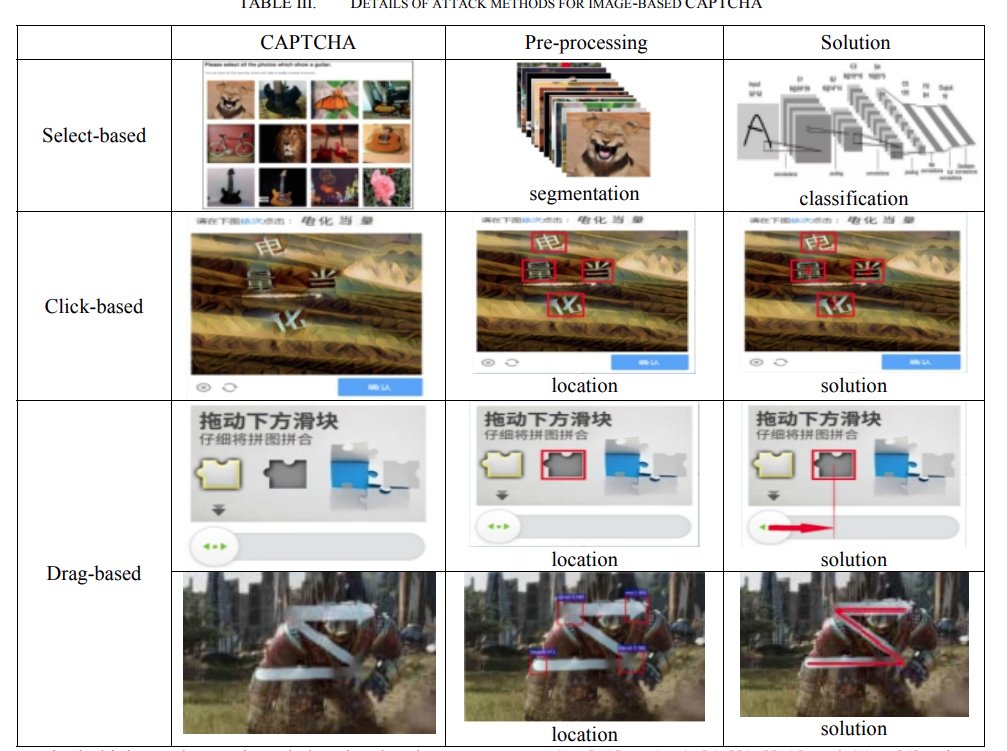
\includegraphics{gfx/mygraphics/unbedingtaustauschen2.png}
    \caption{bildbasierte Beispiele die ich unbedingt noch austauschen muss, weil sie aus \cite{surveyofresearch} sind}
    \label{fig:pr0grammcaptcha}
\end{figure}

\subsection{Alternativen zu klassischen CAPTCHA}
%anti spam plugins
%multi faktor authentifikation
%biometrie
Eine weitere Alternative zu klassischen CAPTCHA sind sogenannte Honeypots. 
Geprägt wurde der Begriff erstmals im Kalten Krieg als Spionagetechnik eingesetzt wurde. \cite[p.2]{joshi:2011} 

Auch heute werden Honeypots eingesetzt, und zwar in der IT-Sicherheit. 
Oft werden sie mit ``Fallen'' assoziiert, welche Hacker anlocken sollen. 
Dadurch können Angriffsarten analysiert werden und ''echte'' Systeme werden nicht angegriffen.

Doch auch im Kontext der Unterscheidung von Menschen und Maschine gibt es Honeypots. 
So kann man HTML-Inputfelder durch CSS verstecken, sodass diese nur durch Bots, welche den Quellcode der Seite scannen, ausgefüllt werden 
und nicht durch Menschen, da diese das Textfeld nicht sehen. 
Bei der Prüfung der Inputs kann nun überprüft werden, ob ein Bot in die Falle getappt ist. 
Nachzulesen sind solche Verfahren in verschiedenen Blogposts, wie \cite{perry:2019}.


\section{UX}

Die Abkürzung UX steht für \textbf{U}ser E\textbf{x}perience und beschreibt die Erfahrungen eines Users bei der Nutzung eines Systems. 
Das Ziel ist, diese Nutzererfahrung möglichst positiv zu halten. 
Im Kontext dieser Ausarbeitung wird die Definition des  ``international standard on ergonomics of human-system interaction'' $($ISO 9241-210$)$
aus dem Jahre 2010 verwendet. 
Diese definitiert UX als die Wahrnehmungen und Resonanzen einer Person, 
welche aus der $($voraussichtlichen$)$ Nutzung eines Produkts, Systems oder Services entstehen. \cite[p.1629]{berni_borgianni_2021}

Die Nutzererfahrung bei der Wahl und Nutzung von CAPTCHA ist neben der Sicherheit ein essentieller Bestandteil.
Bei der Entwicklung einer Bewertungsmatrix soll deshalb hier der Hauptfokus liegen.
Denn wenn ein CAPTCHA schwierig zu lösen ist, oder von bestimmten Personengruppen gar nicht bearbeitet werden kann, so stört dies nicht nur den Nutzungsfluss,
sondern führt gegebenenfalls auch dazu, dass Nutzer*innen die Seite verlassen, ohne ihre gewünschte Aktion zu vollenden. 

%\cite{surveyofresearch}
